\documentclass[../main.tex]{subfiles}

\graphicspath{{\subfix{../img/}}}

\newcommand{\spazio}{\vspace{1em} \newline}

\begin{document}
   \part{Logica del Primo Ordine}

   \chapter{Logica}

   \section{Intuizione}
   Fino ad ora abbiamo incontrato solo la logica proposizionale che purtroppo pecca per quanto riguarda il potere espressivo.\\
   La difficoltà più grande è che possiamo espremire solo insiemi finiti.\\

   \subsubsection{Caratteristiche della logica del primo ordine}
   \begin{itemize}
      \item Termini complessi e formule complesse.
      \item Le formule primitive molte volte non sono parte del linguaggio.
      \item Termini e formule atomiche sono interpretate su un dominio di fatti e entità.\\
         Le formule complesse sono interpretate attraverso un dominio di giudizi.
      \item Le formule complesse sono formate un qualsiasi numero di connettivi proposizionali più un numero di quantificatori.
      \item I quantificatori sono: $\forall$ e $\exists$.
   \end{itemize}

   \subsubsection{Esempi di espressività}
   Come posso esprimere le seguenti frasi?
   \begin{itemize}
      \item Mary is a person.
      \item John is a person.
      \item Mary is mortal.
   \end{itemize}
   Visto che sono proposizioni atomiche non primitive:
   \begin{itemize}
      \item Person(Mary)
      \item Person(John)
      \item Mortal(Mary)
   \end{itemize}
   \vspace{1em}
   La logica del primo ordine risulta più utile nei seguenti casi:
   \begin{itemize}
      \item All people are mortal.
      \item There is (at least) a person who is a spy.
   \end{itemize}
   Che posso esprimere come:
   \begin{itemize}
      \item $\forall$ people.Mortal(people)
      \item $\exists$ person.Spy(person)
   \end{itemize}
   \vspace{1em}
   Con la logica del primo ordine posso anche annidare formule.
   \begin{itemize}
      \item The father of Luca is Italian.
   \end{itemize}
   Diventa:
   \begin{itemize}
      \item Italian(fatherOf(Luca))
   \end{itemize}
   \vspace{1em}
   Infine posso usare i concatenatori visti nella logica proposizionale.
   \begin{itemize}
      \item Every Natural number is either even or odd.
   \end{itemize}
   La posso vedere come:
   \begin{itemize}
      \item $\forall$ number.(odd(number) $\lor$ even(number))
   \end{itemize}

   \section{Sintassi}
   La sintassi di un linguaggio $L$ è definita come segue:
   \begin{itemize}
      \item Un insieme di termini primitivi detti termini alfabetici.
      \item Un insieme di regole per la formazione di formule che permettono di comporre termini atomici.
      \item Un insieme di regole da termine a frase.
      \item Un insieme di frasi primitive chiamato alfabeto delle frasi.
      \item Un insieme di regole per la formazione di frasi.
      \item Un insieme di regole da frasi a termini.
   \end{itemize}

   \subsection{Definizioni}
   \begin{itemize}
      \item \textbf{Alfabeto:} L'alfabeto della logica del primo ordine è formato da due insimi di simboli simboli logici e simboli non logici.
      \item \textbf{Simboli logici:} I simboli logici sono i seguenti:
         \begin{itemize}
            \item In modo opzionale le costanti logiche $\perp$ e $\top$.
            \item In modo opzionale il simbolo di ugualgianza $=$.
            \item Connettivi della logica proposizionale $\land$, $\lor$, $\supset$, $\lnot$, $\equiv$.
            \item Quantificatori $\forall$ e $\exists$.
            \item Un insieme infinito di simboli per le variabili $x_1, x_2, \dots$
         \end{itemize}
      \item \textbf{Simboli non logici:} I simboli non logici sono i seguenti:
         \begin{itemize}
            \item Un insieme di costanti $c_1, c_2, \dots$
            \item Un insieme di funzioni con la loro arietà $f_1, f_2, \dots$
            \item Un insieme di predicati $P_1, P_2, \dots$
         \end{itemize}
      \item \textbf{Termini:}
         \begin{itemize}
            \item Ogni costante $c_i$ e variabile $x_i$ è un termine.
            \item Se $t_1 \dots t_n$ sono termini e $f_i$ una funzione che ha nella firma $n$ elementi, allora $f(t_1 \dots t_n)$ è un termine.
         \end{itemize}
      \item \textbf{Well-formed formulas}
         \begin{itemize}
            \item Se $t_1 \dots t_n$ sono termini e $P$ è un simbolo di relazione con arietà uguale a $n$, allora $P(t_1 \dots t_n)$ è una formula atomica.
            \item Se A e B sono formule allora $\top$, $\perp$, A$\land$B, A$\lor$B, A$\supset$B, $\lnot$A e A$\equiv$B sono formule.
            \item Se A è uina formula e $x$ una variabile allora $\forall x$.A e $\exists x$.A sono fomrule.
         \end{itemize}
   \end{itemize}

   \section{Funzione di interpretazione}
   \textbf{Interpretazio2ne FOL:} Una interpretazione del primo ordine per il linguaggio:
   \begin{center}
      $L=(c_1,c_2, \dots, f_1,f_2, \dots, P_1,P_2, \dots)$
   \end{center}
   è la tupla
   \begin{center}
      $\langle \Delta, I \rangle$
   \end{center}
   Dove:
   \begin{itemize}
      \item $\Delta$ è un insieme non vuoto chiamato \textbf{dominio di interpretazione}.
      \item $I$ è una funzione chiamata \textbf{funzione di interpretazione} definita come:
      \begin{itemize}
         \item $I(c_i) \in \Delta$ (elemento del dominio)
         \item $I(f_i) : \Delta^n \to \Delta$ (n-aria funzione sul dominio)
         \item $I(P_i) \subseteq \Delta^n$ (n-aria relazione sul dominio)
      \end{itemize}
   \end{itemize}
   dove:
   \begin{itemize}
      \item $n$ è l'arietà di $f_i$ e $P_i$
      \item $\Delta^n = \Delta \times \dots \times \Delta$ 
   \end{itemize}

   \subsection{Interpretazione di ground formulas (formule senza variabili)}
   L'interpretazione di un termine è un' entità nel dominio, possiamo avere sinonimità ma non polisemia.\\
   I simboli di funzione sono usati per generare la descrizione di termini complessi, i simboli di una funzione n-aria denotano lo spazio di tutti i possibili termini.\\
   Le entità generate da una funzione n-aria sono rappresentati come una (n+1)-aria tupla.\\
   Predicati n-ari sono usati per generare formule atomiche, i fatti generati da un predicato n-ario sono rappresentati da un tupla n-aria.

   \subsection{Interpretazione di una formula con variabili}
   Una variabile presente in una formula atomica non può essere interpretata come elemento del dominio, nello stesso momento ad una formula atomica deve essere assegnata un'interpretazione.\\
   Possiamo interpretare una variabile come qualcosa la cui interpretazione ci è ancora ignota ma, che in seguito potrà avere un valore compreso nel dominio.\\
   \textbf{N.B.} nessun valore del dominio può essere scartato a priori.

   \subsubsection{Assegnamento delle variabili}
   Sia $L$ un linguaggio del primo ordine e $\Delta$ il suo dominio di interpretaione.\\
   Sia A$\in L$ una formual del primo ordine e Var(A)=\{$x_1, \dots , x_n$\} l'insieme delle variabili occorenti in A.\\
   Un assegnamento $a$ è una funzione dall'insieme delle variabili al dominio di interpretazione $\Delta$:
   \begin{center}
      $a: \text{Var(A)} \to \Delta$
   \end{center}
   Scriveremo $a[x/d]$ per inidcare l'assegnamento $a$ su tutte le variabili tranne $x$ che sono associate a $d$ con $d \in \Delta$.

   \section{Conseguenza logica}
   Siano $L$ un linguaggio formale, $T \subseteq L$ una teoria formale, $I : L \to D$ una funzioane di interpretazione per $L$, $M \subseteq D$ un modello per $T$.\\
   Allora $\models_L$ associa cosa c'è di vero in $M$ con le wffs in $T$:
   \begin{center}
      $\models_L \subseteq M \times T$
   \end{center}
   Possiamo anche scrivere:
   \begin{center}
      $M \models_L T$
   \end{center}

   \subsection{Occorenze libere delle variabili}
   \textbf{Occorrenza libera:} una variabile occurre libermanete se vale una delle seguenti affermaioni:
   \begin{itemize}
      \item Un'occorrenza di $x$ in un termine $t_k$ è libera in $P(t_1, \dots , t_k, \dots , t_n)$.
      \item Ogni occorenza libera di $x$ in una formula $\phi$ o $\psi$ rimane liber anche in $\phi \land \psi$, $\phi \land \psi$, $\phi \supset \psi$, $\phi \equiv \psi$ e $\lnot \phi$.
      \item un'occorrenza libera di $x$ in una formula $\phi$ rimane libera in $\forall y.\phi$ e $\exists y.\phi$ se $y$ è diversa da $x$.
   \end{itemize}
   \textbf{Ground formula:} una formula si dice grounded se non presenta variabili.\\
   \textbf{Closed formula:} una formula si dice chiusa se non contiene occorrenze libere di una variabile.

   \subsection{Soddisfacibilità con riferimento all'assegnamento}
   Un'interpretazione $I$ soddisfa una formula $\phi$ considerando un assegnamento $a$ secondo le seguenti formule:
   \begin{center}
      \begin{tabular}{c c c}
         $I \models t_1 = t_2[a]$ & iff & $I(t_1)[a]=I(t_2)[a]$\\
         $I \models P(t_1, \dots, t_n)[a]$ & iff & $<I(t_1)[a], \dots, I(t_n)[a] > \in I(P)$\\
         $I \models (\phi \land \psi)[a]$ & iff & $I \models \phi[a]\ \text{and}\ I \models \psi[a]$\\
         $I \models (\phi \lor \psi)[a]$ & iff & $I \models \phi[a]\ \text{or}\ I \models \psi[a]$\\
         $I \models (\phi \supset \psi)[a]$ & iff & $I \not \models \phi[a]\ \text{or}\ I \models \psi[a]$\\
         $I \models \lnot \phi[a]$ & iff & $I \not \models \psi[a]$\\
         $I \models (\phi \equiv \psi)[a]$ & iff & $I \models \phi[a]\ \text{iff}\ I \models \psi[a]$\\
         $I \models \exists x \phi[a]$ & iff & $\text{there is a}\ d \in \Delta\ \text{such that}\ I \models \phi[a[x/d]]$\\
         $I \models \forall x \phi[a]$ & iff & $\text{for all}\ d \in \Delta, I \models \phi[a[x/d]]$
      \end{tabular}
   \end{center}

   \subsection{Soddisfacibilità}
   \textbf{Modello rispetto all'assegnamento:} un interpretazione $I$ è un modello di $\phi$ secondo l'assegnamento $a$ se:
   \begin{center}
      $I \models \phi [a]$
   \end{center}
   \textbf{Modello, soddisfacibilità:} un interpretazione $I$ è un modello per $\phi$ se esiste un assengamento $a$ tale che $I$ sia un modello per $\phi$ secondo $a$, una fomrula $\phi$ è soddisfacibile se esiste una qualsiasi $I$ e una $a$ tale che $I \models \phi [a]$.
   \spazio
   \textbf{Implicazione, verità, soddisfacibilità:} le seguenti affermazioni sono equivalenti all'enuinciato $I \models A$:
   \begin{itemize}
      \item La funzione di interpretazione (e anche modello) $I$ implica la formula $A$.
      \item La formula $A$ è vera nella funzione di interpretazione (e anch modello) $I$.
      \item La formula $A$ è soddisfatta dall'interpretaione (e modello) $I$.
   \end{itemize}

   \chapter{Modeling}
   \section{Teoremi principali}
   \subsection{Quantificatori e connettivi proposizionali}
   \begin{itemize}
      \item $\forall x.(\phi (x) \land \psi (x)) \equiv \forall x .\phi (x) \land \forall x. \psi (x)$ è valida
      \item $\exists x.(\phi (x) \lor \psi (x)) \equiv \exists x. \phi (x) \lor \exists x. \psi (x)$ è valida
      \item $\forall x.(\phi (x) \lor \psi (x)) \equiv \forall x. \phi (x) \lor \forall x. \psi (x)$ non è valida 
      \item $\exists x.(\phi (x) \land \psi (x)) \equiv \exists x.\phi (x) \land \exists x. \psi (x)$ non è valida
      \item $\forall x.\phi(x) \equiv \lnot \exists x.\lnot \phi(x)$ è valida
      \item $\forall x.\exists x.\phi(x) \equiv \exists x.\phi(x)$ è valida
      \item $\exists x.\forall x.\phi(x) \equiv \forall x.\phi(x)$ è valida
      \item $\forall x.\phi(x) \equiv \exists x.\phi(x)$ non è valida 
      \item $\forall x\exists y.\phi(x, y) \equiv \exists y\forall x.\phi(x, y)$ non è valida 
   \end{itemize}

   \subsection{Termini liberi per una variabile in una formula}
   Sia $x$ una variabile occorente in un termine $t$, allora $t$ è libero rispetto alla variabile $x$ in una formula $\phi$ se e solo se tutte le occorrenze di $x$ non occorrono in $\phi$ all'interno dello scope del quantificatore, quindi se tutte le occorenze di $x$ in $\phi$ sono libere.

   \section{Errori nella formalizzazione}
   \begin{itemize}
      \item \textbf{$\supset$ and $\forall$:} lo scope di un quantificatore universale può essere indebolito facendolo diventare la conseguenza di un implicazione dove la premessa (dell' implicazione) riduce lo scope.\\
         \textbf{Esempio:} la formula:
         \begin{center}
            $\forall x(\text{WorksAt(UniTn, }x) \supset \text{Smart(}x))$
         \end{center}
         Vuol dire:
         \begin{center}
            "Everybody working at UniTn is smart"
         \end{center}
         Se avessi usato una congiunzione avrei rafforzato la formula anzichè ristretto lo scope:
         \begin{center}
            $\forall x(\text{WorksAt(UniTn, }x) \land \text{Smart(}x))$
         \end{center}
         Vuol dire:
         \begin{center}
            "Everybody works at UniTn and everyone is smart"
         \end{center}
      \item \textbf{$\land$ and $\exists$:} lo scope di un quantificatore di esistenza può essere indebolito aggiungendo una congiunza, la quale aggiungerà un nuovo voncolo da rispettare.\\
         \textbf{Esempio:} la formula:
         \begin{center}
            $\exists x(\text{WorksAt(UniTn, }x) \land \text{Smart(}x))$
         \end{center}
         Vuol dire:
         \begin{center}
            "There is a person working at UniTn and she is smart"
         \end{center}
         Se avessi usato una implicazione avrei rafforzato la formula perchè partendo con una premessa vera l'interpretazione ha più modi di essere vera:
         \begin{center}
            $\exists x(\text{WorksAt(UniTn, }x) \supset \text{Smart(}x))$
         \end{center}
         Vuol dire:
         \begin{center}
            "There is a person so that if (s)he works at UniTn then (s)he is smart"
         \end{center}
      \item \textbf{Esiste almeno $1$:} l'esistenza non pone alcun limite inferiore se devo prendere domini diversi.\\
         \textbf{Esempio:} Proviamo a scrivere la formula "There are at least two students attending the Logic class":
         \begin{center}
            $\exists x_1 \exists x_2( \text{attend}(x_1,\text{Logic}) \land \text{attend}(x_2,\text{Logic}))$
         \end{center}
         Ma la formula così scritta non garantisce che $x_1$ e $x_2$ siano distinti, per cui dobbiamo specificarlo.
         \begin{center}
            $\exists x_1 \exists x_2( \text{attend}(x_1,\text{Logic}) \land \text{attend}(x_2,\text{Logic}) \land x_1 \neq x_2)$
         \end{center}  
      \item \textbf{Esietono almeno $n$:} in generale per garantrire che $n$ elementi siano diversi usando l'esistenza dobbiamo avere una formula della seguente forma ($\phi$ sarà la formula da soddisfare):
         \begin{gather*}
            \exists x_1 \dots x_n (\bigwedge^{n}_{i=1}{\phi (x_i)} \land \bigwedge^{n}_{i \neq j=1}{x_j \neq n_i})
         \end{gather*}
      \item \textbf{Esistono al più $n$:} il quantificatore universale, invece, non impone un limite superiore.\\
         Per poter garantire un numero massimale forziamo che differenti quantificatori universali indichino lo stesso elemento ($\phi$ è la funzione da soddisfare).
         \begin{gather*}
            \forall x_1 \dots x_{n+1} (\bigwedge^{n+1}_{i=1}{\phi (x_i)} \supset \bigvee^{n+1}_{i \neq j=1}{x_j = n_i})
         \end{gather*}
   \end{itemize}

   \chapter{Calculus}
   \section{Nozioni basiche}
   \textbf{Soddisfacibilità con riferimento ad un assegnamento:} un'interpretazione $I$ soddisfa una formula $\phi$ con un assegnamento $a$ secondo le seguenti formule:
   \begin{center}
      \begin{tabular}{c c c}
         $I \models t_1 = t_2 [a]$ & iff & $I(t_1)[a]=I(t_2)[a]$\\
         $I \models P(t_1, \dots ,t_n)[a]$ & iff & $< I(t_1)[a], \dots , I(t_n)[a] > \in I(P)$\\
         $I \models (\phi \land \psi)[a]$ & iff & $I \models \phi[a] and I \models \psi[a]$\\
         $I \models (\phi \lor \psi)[a]$ & iff & $I \models \phi[a] or I \models \psi[a]$\\
         $I \models (\phi \supset \psi)[a]$ & iff & $I \not \models \phi [a] or I \models \psi[a]$\\
         $I \models \lnot \phi[a]$ & iff & $I \not \models \phi[a]$\\
         $I \models (\phi \equiv \psi)[a]$ & iff & $I \models \phi[a] iff I \models \psi[a]$\\
         $I \models \exists x \phi[a]$ & iff & there is a $d \in \Delta$ such that $I \models \phi[a[x/d]]$\\
         $I \models \forall x \phi[a]$ & iff & for all $d \in \Delta, I \models \phi[a[x/d]]$
      \end{tabular}
   \end{center}
   \textbf{Modello rispetto ad un assegnamento:} un'interpretazione $I$ è un modello di $\phi$ secondo un'assegnamento $a$ se:
   \begin{center}
      $I \models \phi[a]$
   \end{center}
   \textbf{Insoddisfacibile:} una formula è insoddisfacibile se non è soddisfacibile.
   \spazio
   \textbf{Validità:} una formula $\phi$ è valida se per ogni interpretazione $I$ e ogni assegnamento $a$ vale che:
   \begin{center}
      $I \models \phi[a]$
   \end{center}
   Nella logica del primo ordine valgono le stesse proprietà della logica proposizionale, quindi:
   \begin{center}
      Valida $\supset$ Soddisfacibile $\supset \lnot$ Insoddisfacibile\\
      \vspace{4ex}
      Insoddisfacibile $\supset \lnot$ Soddisfacibile $\supset \lnot$ Valida\\
      \vspace{4ex}
      \begin{tabular}{c c}
         \hline
         se A è & allora $\lnot$ A è\\
         \hline
         \hline
         Valida & Insoddisfacibile\\
         Soddisfacibile & $\lnot$ Valida\\
         $\lnot$ Valida & Soddisfacibile\\
         Inddisfacibile & Valida
      \end{tabular}
   \end{center}
   \textbf{Conseguenza logica:} una formula $\phi$ è una conseguenza logica di un insieme di formule $\Gamma$  se per ogni interpretazione $I$ e ogni assegnamento $a$
   \begin{center}
      $I \models \Gamma [a]$ implica $I \models \phi [a]$
   \end{center}
   dove $I \models \Gamma [a]$ significa che $I$ soddisfa tutte le formule di $\Gamma$ sotto $a$.
   \spazio
   \textbf{Equivalenza logica:} due formule $\phi$ e $\psi$ sono logicamente equivalente se e solo se $\phi \models \psi$ e $\psi \models \phi$, scriveremo:
   \begin{center}
      $\models \phi \equiv \psi$
   \end{center}
   \textbf{Teorema di deduzione:} $\Gamma , \phi \models \psi$ se e solo se $\Gamma \models \phi \supset \psi$.
   \spazio
   \textbf{Principio di refutazione:} $\Gamma \models \phi$ se e solo se $\Gamma \cup \{ \lnot \phi \}$ è insoddisfacibile.
   \spazio
   \textbf{Formule chiuse:} nelle formule chiuse validità, soddisfacibilità, insoddisfacibile, conseguenza logica e equivalenza logica non dipendono dall'assegnamento, infatti nella notazione scriveremo solo $\phi$ anzichè $\phi[a]$.
   \spazio
   \textbf{Invarianza dell'assegnazione:} siano $[a^1]$ e $[a^2]$ due assegnamenti allora $I \models [a^1]$ se e solo se $I \models [a^2]$ quando $[a^1]$ e $[a^2]$ coincidono in una variabile libera in $\phi$.

   \chapter{Inferenza della DPLL}
   \section{Dominio finito}
   \textbf{Estensione finita del predicato:} questa assunzione enuncia che un predicato $P$ è vero solo per un sottoinsieme finito del proprio dominio originale.\\
   L'assunzione può essere formalizzata nella formula:
   \begin{center}
      $\forall x(P(x) \equiv (x=c_1 \lor \dots \lor x=c_n))$
   \end{center}
   \textbf{Assunzione del nome univoco:} un linguaggio deve contenere uno e un solo nome per ogni elemento del dominio, assumendo che un linguaggio contenga le costanti $c_1, \dots , c_n$ abbiamo:
   \begin{gather*}
      \phi_\Delta = \{ c_1, \dots , c_n \}\\
      \vspace{4ex}
      \{ c_1, \dots , c_n \} = \biggl( \bigwedge_{i \neq j=1}^{n}{c_i \neq c_j} \land \forall x \biggl( \bigvee_{i=1}^{n}{c_i=x} \biggr) \biggr)
   \end{gather*}
   \textbf{Espansione dei quantificatori:} secondo l'ipotesi di un dominio finito con dei nomi univoci la logica del primo ordine può essere proposizionalizzata secondo le seguenti equivalenze:
   \begin{itemize}
      \item $\phi_\Delta = \{ c_1, \dots , c_n \} \models \forall x.\phi(x) \equiv \phi(c_1) \land \dots \land \phi(c_n)$
      \item $\phi_\Delta = \{ c_1, \dots , c_n \} \models \exists x.\phi(x) \equiv \phi(c_1) \lor \dots \lor \phi(c_n)$
   \end{itemize}
   \textbf{Esempio:} prendiamo la formula in linguaggio naturale "Everybody living in Toulouse speak french or spanish", tradotta in FOL risulta in:
   \begin{center}
      $\forall x.( \text{Lives}( x,\text{Toulouse} ) \supset ( \text{Speaks}( x,\text{French} ) \lor \text{Speaks}( x,\text{Spanish} ) ) )$
   \end{center}
   Assumiamo che l'insieme delle persone sia:
   \begin{center}
      $\Delta_1=$\{Robert, Luis, Naji\}
   \end{center}
   Allora possiamo rendere ground la precende formula, e riscriverla come segue:
   \begin{center}
      (Lives(Robert,Toulouse) $\supset$ Speaks(Robert,French) $\lor$ Speaks(Robert,Spanish)) $\land$\\
      (Lives(Luis,Toulouse) $\supset$ Speaks(Luis,French) $\lor$ Speaks(Luis,Spanish)) $\land$\\
      (Lives(Naji,Toulouse) $\supset$ Speaks(Naji,French) $\lor$ Speaks(Naji,Spanish)) 
   \end{center}
   \textbf{Esempio:}  prendiamo la formula in linguaggio naturale "If someone is noisy, everyone is annoyed", tradotta in FOL risulta:
   \begin{center}
      $\exists x.( \text{Noisy}(x) \supset \forall y.( \text{Annoyed}(y) ) )$
   \end{center}Assumiamo che l'insieme delle persone sia:
   \begin{center}
      $\Delta_1=$\{Marco, Francesco, Pierre\}
   \end{center}
   Allora possiamo rendere ground la precende formula, e riscriverla come segue (\textbf{N.B.} non viene detto che $x \neq y$):
   \begin{center}
      (Noisy(Marco) $\supset$ Annoyed(Marco) $\land$ Annoyed(Francesco) $\land$ Annoyed(Pierre)) $\lor$\\
      (Noisy(Francesco) $\supset$ Annoyed(Marco) $\land$ Annoyed(Francesco) $\land$ Annoyed(Pierre))$\lor$\\
      (Noisy(Pierre) $\supset$ Annoyed(Marco) $\land$ Annoyed(Francesco) $\land$ Annoyed(Pierre))
   \end{center}

   \section{PNF - Prenex Normal Form}
   \textbf{Prenex Normal Form:} una formula in logica del primo ordine si dice essere in PNF se ha la seguente forma:
   \begin{center}
      $Q_1 x_1 Q_2 x_2 \dots Q_n x_n .P$
   \end{center}
   dove:
   \begin{itemize}
      \item $Q_i$ è un quantificatore di esistenza o universale.
      \item La o del punto precedente è esclusiva.
      \item $P$ è un quantificatore libero.
   \end{itemize}
   $Q_1 x_1 Q_2 x_2 \dots Q_n x_n$ è detto prefisso mentre $P$ è la matrice.
   \spazio
   Ogni formula di logica del primo ordine può essere scritta in PNF.
   \spazio
   \textbf{Passi della PNF:}
   \begin{itemize}
      \item Muovere le negazionbi all'interno finchè non ci saranno più quantificatori nello scope di una negazione.
      \item Rinominare le variabili finchè ogni variabile che segue un quantificatore avrà un nome univoco.
      \item Muovere all'esterno i quantificatori leggendo la formula da sinistra a destra.
   \end{itemize}
   \begin{center}
      \begin{tabular}{c c c c}
         \textbf{Formula} & & \textbf{versione PNF} & \textbf{Assunzioni}\\
         \hline
         $\lnot \forall x.\phi x$ & $\equiv$ & $\exists x.(\lnot \phi (x))$ & \\
         $\lnot \exists x.\phi x$ & $\equiv$ & $\forall x.(\lnot \phi (x))$ & \\
         $\forall x.(\phi (x)) \land \psi$ & $\equiv$ & $\forall x.(\phi (x) \land \psi)$ & $\forall x.\top$\\
         $\exists x.(\phi (x)) \land \psi$ & $\equiv$ & $\exists x.(\phi (x) \land \psi)$ & $\exists x.\top$\\
         $\forall x.(\phi (x)) \lor \psi$ & $\equiv$ & $\forall x.(\phi (x) \lor \psi)$ & $\forall x.\top$\\
         $\exists x.(\phi (x)) \lor \psi$ & $\equiv$ & $\exists x.(\phi (x) \lor \psi)$ & $\exists x.\top$\\
         $\forall x.(\phi (x)) \supset \psi$ & $\equiv$ & $\exists x.(\phi (x) \supset \psi)$ & $\exists x.\top$\\
         $\exists x.(\phi (x)) \supset \psi$ & $\equiv$ & $\forall x.(\phi (x) \supset \psi)$ & $\forall x.\top$\\
         $\psi \supset \forall x.(\phi (x))$ & $\equiv$ & $\forall x.(\psi \supset \phi (x))$ & $\forall x.\top$\\
         $\psi \supset \exists x.(\phi (x))$ & $\equiv$ & $\exists x.(\psi \supset \phi (x))$ & $\exists x.\top$
      \end{tabular}
   \end{center}
   \vspace{4ex}
   \textbf{Proposizione:} ogni formula in PNF con la forma $\exists x_1 \exists x_2 \dots \forall x_{n-1} \forall x_n .P$ tale che:
   \begin{itemize}
      \item La sua matrice non contenga alcuna funzione e \dots
      \item I suoi prefissi sono composti da una serie (anche vuota) di quantificatori di esistenza e una serie (anche vuota) di quantificatori universali.
   \end{itemize}
   è deducibile quindi valida/soddisfacibile/insoddisfacibile.

   \section{DPLL in FOL}
   Adesso abbiamo una formula in FOL che abbiamo trasformato in PNF e a cui abbiamo "ristretto" il dominio per farla diventare una formula in PL.\\
   Essendo una formula in PL possimao applicare le formule per scriverla in CNF e poter applicare DPLL.
   \begin{align*}
      CNF(p)&=\text{p se p} \in \textbf{PROP}\\
      CNF(\lnot p) &=\text{$\lnot$p se p} \in \textbf{PROP}\\
      CNF(\phi \supset \psi) &= CNF(\lnot \phi) \otimes CNF(\psi)\\
      CNF(\phi \land \psi) &= CNF(\phi) \land CNF(\psi)\\
      CNF(\phi \lor \psi) &= CNF(\phi) \otimes CNF(\psi)\\
      CNF(\phi \equiv \psi) &= CNF(\phi \supset \psi) \land CNF(\psi \supset \phi)\\
      CNF(\lnot \lnot \phi) &= CNF(\phi)\\
      CNF(\lnot (\phi \supset \psi)) &= CNF(\phi) \land CNF(\lnot \psi)\\
      CNF(\lnot (\phi \land \psi)) &= CNF(\lnot \phi) \otimes CNF(\lnot \psi)\\
      CNF(\lnot (\phi \lor \psi)) &= CNF(\lnot \phi) \land CNF(\lnot \psi)\\
      CNF(\lnot (\phi \equiv \psi)) &= CNF(\phi \land \lnot \psi) \otimes CNF(\psi \land \lnot \phi)
   \end{align*}
  Dove $(C_1 \land \dots \land C_n) \otimes (D_1 \land \dots \land D_m)$ è definito come:
  \begin{center}
      $(C_1 \lor D_1) \land \dots \land(C_1 \lor D_m) \land \dots \land(C_n \lor D_1) \land \dots \land(C_n \lor D_m)$
  \end{center}

  \subsubsection{Esempio}
  Abbuiamo la frase:
  \begin{center}
      A mechanic likes herself
  \end{center}
  Tradotta in FOL risulta essere:
  \begin{center}
      $\exists x.(\text{Mechanic}(x) \land \text{Likes}(x, x))$
  \end{center}
  Poniamo come dominio sottoinsieme del dominio $\Delta=$\{Amanda, Miriam\}, quindi la formula ground risulta essere:
  \begin{center}
      $\psi = p \land q \lor p_1 \land q_1$
  \end{center}
  Adesso che abbiamo una formula in PL possiamo riscriverla in CNF per applicare DPLL e vedere se è soddisfacibile.
  \begin{align*}
      (p \land q) & \lor (p_1 \land q_1)\\
      (p \land q)  & \otimes (p_1 \land q_1)\\
      (p \lor p_1) \land (p \lor q_1) & \land (q \lor p_1) \land (q \lor q_1)\\
      ( \top \lor p_1) \land ( \top \lor q_1) & \land (q \lor p_1) \land (q \lor q_1)|_p\\
      (q \lor p_1) & \land (q \lor q_1)\\
      ( \top \lor p_1) & \land ( \top \lor q_1)|_q
  \end{align*}

  \chapter{Inferenza dei Tableaux}
  \section{Tableaux del primo ordine}
  \textbf{Tableaux del primo ordine:} è un albero radicato, ogni suo nodo contiene una frase in FOL.

  Il figlio di un nodo $n$ è generato applicando una serie di regole di espansione a $n$ o a uno degli antenati di $n$.
  \spazio
  Il metodo del tablueaux è composto da 3 elementi:
  \begin{itemize}
      \item Un dato insieme di premesse $\Gamma$ e conclusioni $\phi$.
      \item \textbf{Un compito:} provare che $\Gamma \models \phi$.
      \item \textbf{Procedura:} mostrare che $\Gamma \cup \{ \lnot \phi \}$ è non soddisfacibile che è equivalente a dimostrare che $\Gamma \cup \{ \phi \}$ è soddisfacibile.
  \end{itemize}
  \subsection{Regole $\alpha$}
  Sono le stesse della logica proposizionale.\\
  \begin{minipage}{0.333333\textwidth}
   \begin{gather*}
       \phi \land \psi\\
       \downarrow\\
       \phi\\
       \psi
   \end{gather*}
   \end{minipage}
   \begin{minipage}{0.333333\textwidth}
      \begin{gather*}
         \lnot (\phi \lor \psi)\\
         \downarrow\\
         \lnot \phi\\
         \lnot \psi
      \end{gather*}
   \end{minipage}
   \begin{minipage}{0.333333\textwidth}
      \begin{gather*}
         \lnot (\phi \supset \psi)\\
         \downarrow\\
         \phi\\
         \lnot \psi
      \end{gather*}
   \end{minipage}
   \subsection{Regole $\beta$}
   Anche le regole $\beta$ sono uguali a quelle delle logica proposizioanale.
   \begin{center}
      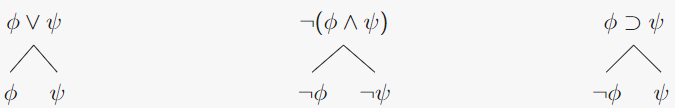
\includegraphics{beta_rules.png}
   \end{center}
   \subsection{Regole $\gamma$}
   \begin{minipage}{0.5\textwidth}
      \begin{gather*}
         \forall x. \phi (x)\\
         \downarrow\\
         \phi (t)
      \end{gather*}
   \end{minipage}
   \begin{minipage}{0.5\textwidth}
      \begin{gather*}
         \lnot \exists x. \phi (x)\\
         \downarrow\\
         \lnot \phi (t)
      \end{gather*}
   \end{minipage}
   Dove $t$ è un nuovo termine libero rispetto a $x$ in $\phi$.
   \subsection{Regole $\sigma$}
   \begin{minipage}{0.5\textwidth}
      \begin{gather*}
         \lnot \forall x. \phi (x)\\
         \downarrow\\
         \lnot \phi (c)
      \end{gather*}
   \end{minipage}
   \begin{minipage}{0.5\textwidth}
      \begin{gather*}
         \exists x. \phi (x)\\
         \downarrow\\
         \phi (c)
      \end{gather*}
   \end{minipage}
   Dove $c$ è una nuova costante non precedentemente apparsa nel tablueaux.
   \subsection{Sostituzione $\phi [x/t]$}
   In questa notazione $x$ è una variabile libera mentre $t$ è un termine, con la notazione $\phi [x/t]$ intendiamo sostituira tutte le occorrenze di $x$ con $t$ in $\phi$.
   \subsubsection{Esempi:}
   \begin{gather*}
      P(x, y, f(x))[x/a] = P(a, y, f (a))\\
       \forall x.P(x, y)[x/b] = \text{Non permesso perchè x non è libera}\\
       \exists x.P(x, x)  \land Q(x)[x/c] =  \exists x.P(x, x)  \land Q(c)\\
      P(x, g(y))[y/f (x)] = P(x, g(f (x)))\\
       \forall x.P(x, y)[y/f (x)] = \text{Non permesso perchè f(x) non è libera per y nello scope di y}
   \end{gather*}
   \subsection{Esempio di Tableaux}
   Verifichiamo ora la validità/soddisfacibilità della seguente formula:
   \begin{center}
      $\phi =  \forall x, y(P(x) \supset Q(y))  \supset ( \exists x.P(x)  \supset  \forall y.Q(y))$
   \end{center}
   Verifichiamo la validità, quindi facciamo il tablueaux per $\lnot \phi$.
   \begin{center}
      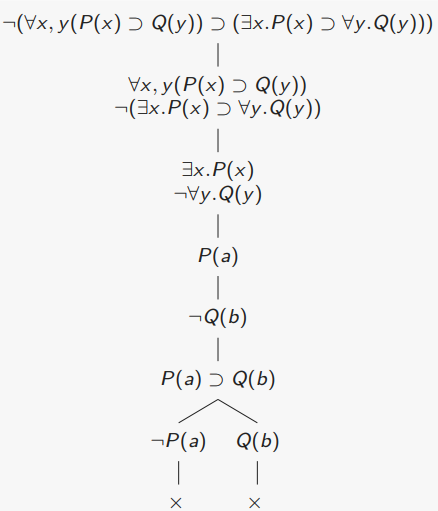
\includegraphics[scale=0.6]{Tableaux_FOL_1.png}
   \end{center}
   \vspace{4ex}
   Verifichiamo ora la validità/soddisfacibilità della seguente formula:
   \begin{center}
      $( \exists x.(P(x)  \lor Q(x))) \equiv (( \exists x.P(x))  \lor ( \exists x.Q(x)))$
   \end{center}
   Verifichiamo la validità, quindi facciamo il tablueaux per $\lnot \phi$.
   \begin{center}
      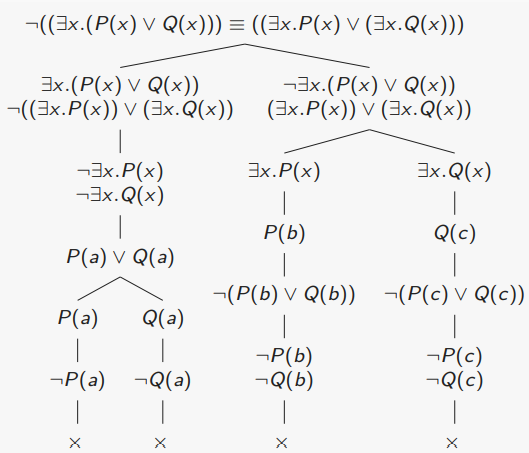
\includegraphics[scale=0.6]{Tableaux_FOL_2.png}
   \end{center}

   \section{Gestione dei Tableaux}
   In questa sezione ci sono tutte le regole di come bisogna espandere un Tableaux.
   \spazio
   \textbf{Espansione dell'esietnza:} se possibile è bene iniziare applicando tutte le regole $\sigma$ per ottenere tutti i termini con cui lavoreremo.
   \spazio
   \textbf{Espansione universale:} dobbiamo applicare le regole $\gamma$ dopo le regole $\sigma$, quando applicate devono matchare i termini già presenti nel Tableaux in particolare matchare le costanti introdotte con le regole $\sigma$.

   Il termine inserito deve essere inserito perchè si verifichi sempre una chiusura del ramo.

   \subsubsection{Esempio}
   Verifichiamo se $\lnot (\forall x.P(x) \land \exists x. \lnot P(f(x)))$ è valida/soddisfacibile/insoddisfacibile.
   \begin{gather*}
      \forall x.P(x) \land \exists x. \lnot P(f(x))\\
      \downarrow\\
      \forall x.P(x)\\
      \exists x. \lnot P(f(x))\\
      \downarrow\\
      \lnot P(f(c))\\
      \downarrow\\
      P(f(c))\\
      \downarrow\\
      \times
   \end{gather*} 

   \subsection{Non-terminazione}
   A differenza della logica proposizionale in FOL i modelli possono essere infiniti, esistono infatti formule soddisfatte solo da modelli infiniti.\\
   Se cerchiamo di costruire un Tableaux per queste formule in cerca di un modello finiremo in un loop di espansioni.

   \subsubsection{Esempio}
   \begin{center}
      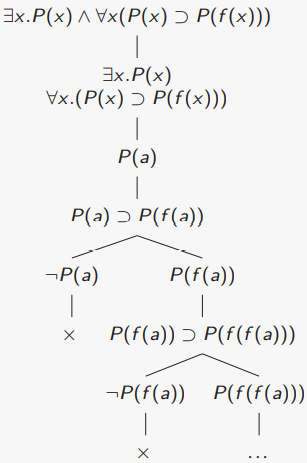
\includegraphics[scale=0.7]{Tableaux_FOL_loop.png}
   \end{center}
   A differenza della logica proposizionale in FOL la costruzione dei Tableaux non assicura di avere una fine.
   \begin{itemize}
      \item Se la formule $\phi$ che indica la radice è insoddisfacibile allora il Tableaux ha una fine e può sempre chiudere.
      \item Se la formule $\phi$ che indica la radice è soddisfacibile la costruzione del Tableaux può finire a rimanere con i rami aperti oppure la costruzione può non terminare mai.
   \end{itemize}
   Ma come facciamo a sapere che siamo in un loop infinito?\\
   Se non abbiamo ancora chiuso un Tableaux è perchè o può essere espanso in modo infinito oppure perchè non abbiamo trovato ancora un modo corretto di costruirlo.\\
   Non possiamo determinarlo.

   \subsection{Contromodello}
   \textbf{Ramo aperto saturato:} un ramo aperto si chiama saturato se ogni non letterale è stato analizzato almeno una volta e ogni formula $\gamma$ è stata istanziata con ogni simbolo, che possiamo costruire con i simboli di funzione, su quel ramo.
   \spazio
   \textbf{Prova fallimentare:} un Tableaux con un ramo aperto e saturo non potrà mai essere chiuso, quindi possiamo fermarci subito e dichiarare quella prova fallimentare.
   \spazio
   Un modello $M$, che è un interpretazione, indica come interpretare costanti (elementi del dominio), funzioni e simboli predicativi.
   \begin{itemize}
      \item Dominio: insieme di tutti i termini che possiamo costruire con i simboli di funzioni che appaiono sul ramo.\\
         E' possibile introdurre una costante fittizia per il valore di un termine.
      \item Simboli di funzione: interpretati come scritti o usando una costante fittizia.
      \item Simboli relazionali: interpretati in termini delle loro occorrenze nel ramo.
   \end{itemize}

   \subsubsection{Esempio}
   \begin{center}
      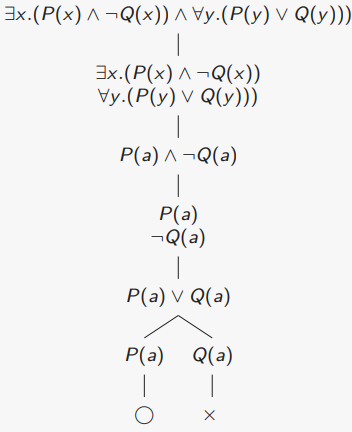
\includegraphics[scale=0.6]{Tableaux_FOL_coutermodel.png}
   \end{center}
   Consideriamo il Tableaux sopra, dalla formula nel ramo aperto è possibile costrire un modello per la formula alla radice.\\
   Per la costruzione del modello prendo:
   \begin{itemize}
      \item $\Delta=$\{a\} la costante apparsa nella formula.
      \item $I(P)$=\{a\} perchè $P$(a) appare nel ramo aperto.
      \item $I(Q)=\{\}$ perchè la formula $\lnot Q(a)$ appare nel ramo aperto.
   \end{itemize}
\end{document}